Transmembrane potentials are due to ion flux accross the membrane. These ion fluxes can be described by the Nernst-Plank equation
\begin{equation}
    J_{total} = J_{diff}+J_{elec} = -D\bigg(\nabla c + \frac{zF}{RT}c\nabla u\bigg)
    \label{nerstplankeq}
\end{equation}
where $J_{total}$ is the total ion flux, $J_{diff}$ is the diffusion flux, $J_{elec}$ is the electric flux, $D$ is the diffusion coefficient and $c$ is the concentration of the ion, $R$ is the ideal gas constant, $T$ is temperature, $F$ is Faraday's constant and $u$ is the electric potential. The Nernst-Plank equation is derived from Fick's law and the Einstein relation, a full derivation can be found in appendix \ref{appendixNPE}. \par
The Nernst-Plank equation can be applied to cellular geometries and used to form the Goldman-Hodgkin-Katz (GHK) current-voltage relation (equation \ref{GHKcvr}) which is used to calculate the ion concentrations and currents discussed in section \ref{cellelectro}
\begin{equation}
    I=P\frac{z^2F^2}{RT}v\frac{c^i-c^eexp\big(\frac{-zvF}{RT}\big)}{1-exp\big(\frac{-zvF}{RT}\big)}
    \label{GHKcvr}
\end{equation}
where $I$ is the electric current density, $P$ is the permeability of the membrane to the ion, $z$ is the valence of the ion and $v = u(0)-u(L) = u_i-u_e$ where $L$ is the membrane length. $c$ is the ion concentration and the $i$ and $e$ notation is used to indicate intra and extracellular values. A full derivation of the GHK current-voltage relation can be found in appendix \ref{appendixGHK}.\par
These equations fundamentally describe the transmembrane potential actions of interest and most models are based of the fundamental relations described by these equations.

\subsection{Equivalent Circuit Model}
An alternative approach to describing the transmembrane potential is by considering electrical circuits. Cells can be described simply as an insulating lipid bilayer membrane with voltage controlled pores known as ion channels. The insulating membrane separates intra and extracellular ion concentration acting as a basic capacitor. The ion channels themselves can be most simply described as resistors (see figure \ref{fig3.1}). If the membrane capacitance ($C_m$) is constant, the current across the membrane ($I_{cap}$) can be described as
\begin{equation}
    I_{cap} = \frac{dQ}{dt} = C_m\frac{dv}{dt}
\end{equation}
were $Q$ is the charge and $v$ is the potential across the membrane. By Kirchhoff's law the total current applied to the membrane, $I_{app}$ is the sum of the membrane capacitance current $I_{cap}$ and the current through the ion channels $I_{ion}$.
\begin{equation}
    I_{app}=C_m\frac{dv}{dt}+I_{ion}
\end{equation}
The structure of the total $I_{ion}$ current is dependent on the specific model employed.

\subsection{Ion Channel Gating}
The current through an ion channel, in general, can be modelled as a product of a function of the number of open channels, $g(v,t)$, and a function of the channels current-voltage relation, $\phi(v)$. $\phi(v)$ can be modelled by various equations as discussed in section \ref{ccmm} on membrane models. The functions $g(v,t)$ can be found experimentally via voltage clamp methods where an external current is applied to a cell to balance the membrane current in a way that keeps the membrane potential $v$ fixed.\par

It is found that the function $g(v,t)$ is related to the number of subunits that make up the ion channel and the kinetics of those subunits. Subunits are the individual complex proteins that make up the channels and pumps. The Hodgkin-Huxley model takes this concept and couples the equivalent circuit model with these gating functions.

\subsection{Hodgkin-Huxley Model}
One of the most celebrated action potential models, the Hodgkin-Huxley (HH) model, combines the equivalent circuit model with gating functions of the form
\begin{equation}
    \frac{dw}{dt} = \frac{w_\infty - w}{\tau_w}
\end{equation}
where $w$ is the gating variable, $w_\infty$ is the equilibrium state and $\tau_w$ is the time constant. \par

The HH model simulates nerve action potentials by using 3 gating variables $m$, $h$ and $n$ to describe the system of the sodium, potassium and leakage currents that make up nerve axon action potentials.
\begin{equation}
    \begin{split}
        & C_m\frac{dv}{dt} + I_{ion}(v,m,h,n) = I_{app} \\
        & \frac{dm}{dt}=\frac{m_\infty(v) - m}{\tau_m(v)} \\
        & \frac{dh}{dt}=\frac{h_\infty(v) - h}{\tau_h(v)} \\
        & \frac{dn}{dt}=\frac{n_\infty(v) - n}{\tau_n(v)} \\
    \end{split}
\end{equation}
and the $I_{ion}$ current is the sum of the individual ion currents and leakage current $I_L$.
\begin{equation}
    I_{ion}=I_{Na}+I_{K}+I_{L}
\end{equation}
It is found that the gating variables are dependent on the number of subunits involved in each channel and their kinetics. The HH approach can be expanded to take into account the larger ionic system involved with cardiac action potentials, leading to a large variety of models for each of the unique cell types of the heart.

\subsection{Cardiac Cellular Membrane Models}
\label{ccmm}

Sophisticated models of individual cell types with a focus on the ionic currents involved have been developed. One of the vital areas of the heart is the sinoatrial node, SAN, which acts as the natural pacemaker. Detailed membrane models have been produced for various animals with noticeable examples being Zhang et al. model of rabbit SAN cells \citep{zhangsan} and Severi et al. model which focuses on calcium ion handling and inhibition which is crucial to the unique plateau in phase 2 of the cardiac cell action potential \citep{severisan}. \par

Atrial tissue models have also been developed such as Nygren et al. human right atrial model which is based on voltage clamp data of isolated cells \citep{nygrenatrial}. Combining HH type equations with a fluid model for intracellular ion movement within the cytoplasm means this model is a very accurate single cell action potential model. The Nygren model and other similar models are embellishments of DiFrancesco and Noble's models of cardiac electrical activity \citep{DiFrancescoNoble}. These models are accurate representations of single cell systems and ion behaviour. \par

The first ventricular model was developed by Beeler and Reuter \citep{beelerreuter}. It was based on the HH model but introduced dynamics necessary to model the effects of calcium ions which are crucial to cardiac action potentials. Many other ventricular models have been developed of varying complexity, a collection of these are shown in table \ref{ventmodletable}. \par

The Beeler and Reuter model along with the Luo and Rudy model were the early attempts to consider calcium ion dynamics. Later models such as Puglisi's model and Shannon's model included more detailed descriptions of the calcium dynamics. Further complexity has been included in more recent models for sodium and potassium ion dynamics and O'Hara and Rudy's model of human ventricular myocytes is particularly detailed.

\begin{table}[h!]
\centering
    \begin{tabular}{||c c c||} 
        \hline
        Model & Species & Equations \\ [0.5ex] 
        \hline\hline
        Beeler \& Reuter \citep{beelerreuter} & Mammalian & 8 \\
        \hline
        Luo \& Rudy \citep{luorudy} & Guinea Pig & 8 \\
        \hline
        Priebe \& Beuckelmann \citep{priebe} & Human & 22 \\
        \hline
        Pandit et al. \citep{pandit} & Rat & 26 \\
        \hline
        Jafri, Rice \& Winslow \citep{JRW} & Guinea Pig & 31 \\
        \hline
        O'Hara \& Rudy \citep{ohararudy} & Human & 41 \\
        \hline
        Shannon et al. \citep{shannon} & Rabbit & 46 \\
        \hline
        Cortassa et al. \citep{cortassa} & Mammalian & 50 \\
        \hline
    \end{tabular}
\caption{A table of some of the most popular ventricular myocyte models. The models are of varying complexity and for different species' dynamic systems.}
\label{ventmodletable}
\end{table}

\subsection{Lightweight Ionic models}
Many of the individual cellular models already mentioned are highly sophisticated and complex. They describe individual cell ion dynamics very well, however, the models themselves are large and mathematically cumbersome, made up of many coupled equations. In order to investigate large multicellular geometries over long temporal scales a reduced model is necessary. These reduced models accurately provide an action potential but without the complex sub-cellular dynamics. This allows for accurate action potential simulation without the computational cost associated with complex models.
\subsubsection{Fitzhugh-Nagumo and Cubic-Like Models}
The Fitzhugh-Nagumo (FN) model is one such example of a lightweight ionic model and is based on a pair of ODEs of the normalised variables $u$, the transmembrane potential, and $v$, the gating variable \citep{fitzhugh}. The equations are based around the form
\begin{equation}
    \begin{split}
        & \frac{du}{dt} = f(u,v) \\
        & \frac{dv}{dt} = g(u,v)
    \end{split}
    \label{FNeq}
\end{equation}
The FN model is one example of cubic-like reduced ionic models and is of the general form 
\begin{equation}
    \begin{split}
        & f(u,v) = -ku(u-a)(u-1)-v \\
        & g(u,v) = \epsilon(u-bv) \\
    \end{split}
\end{equation}
Other cubic-like models have been developed such as the Aliev-Panfilov model \citep{alievpanfilov} and the Mitchell-Schaeffer model \citep{mitchellSchaeffer}. \par

An alternative approach to reduced models is shown in the Fenton-Karma model \citep{fentonkarma}. This consists of three ODEs making up the transmembrane potential, $u$, with two gating variable, $v$ and $w$, as shown in equation \ref{eqFK}.
\begin{equation}
    \begin{split}
        & \frac{du}{dt} = f(u,v,w) \\
        & \frac{dv}{dt} = H(u-u_c)(1-v)/\tau^{-}_{v(u)} - H(u-u_c)v/\tau^{+}{v} \\
        & \frac{dw}{dt} = H(u-u_c)(1-w)/\tau^{-}_{w(u)} - H(u-u_c)w/\tau^{+}{w} \\
    \end{split}
    \label{eqFK}
\end{equation}
where $H$ is the Heaviside function and $f(u,v,w)$ is the sum of the individual membrane ionic currents which can be found experimentally via voltage clamp methods or modelled. \par

Looking at the FN model in more detail, it can be derived from a simple circuit model of a cell membrane. The circuit is made up of a capacitor (current $I_{cap}$) in parallel with a nonlinear current voltage device (current $I_{ion} = F(u)$) and a serial system of a resistor, an inductance, and a voltage source (current $I_0$). Let $u$ equal the transmembrane potential (the difference between the intra, $u_i$, and extra, $u_e$, cellular potentials). Also let $v_R$, $v_L$, and $v_0$ be the resistor, inductor and voltage source potentials. By using Kirchhoff's laws:
\begin{equation}
    \begin{split}
        & I_a = I_{cap} + I_{ion} + I_0 \\
        & u = v_0 + v_L + v_R \\
    \end{split}
\end{equation}
Then by using Ohm's law ($v_R=RI_{ion}$), Faraday's law ($v_L=L\frac{dI_{ion}}{dt}$) and the equation for capacitance ($I_{cap}=C\frac{du}{dt}$) we form
\begin{equation}
    \begin{split}
        & C\frac{du}{dt} = -I_{ion} -F(u) +I_a \\
        & L\frac{I_{ion}}{dt} = u - RI_{ion} - v_0 \\
    \end{split}
\end{equation}
The equation can be made dimensionless by scaling time as $\tau=R_mt/L$, where $R_m=1/F'(0)$. By defining the dimensionless variables as
\begin{equation}
    \begin{split}
        & v(\tau)=u(L\tau/R_m)/u_m \\
        & w(\tau)=R_mI_{ion}(L\tau/R_m)/u_m \\
    \end{split}
\end{equation}
where $u_m$ is the maximum value of $u$. By applying these variables and then defining $\hat v_0=v_0/u_m$, $\hat F(u)=\frac{R_m}{u_m}F(u_mu)$, $\hat I_a=\frac{R_m}{u_m}I_a$, $\gamma = R/R_m$, and $\epsilon = CR^{2}_{m}/L$ gives
\begin{equation}
    \begin{split}
        & \epsilon\frac{du}{d\tau} = -w - \hat F(u) + \hat I_a \\
        & \frac{dw}{d\tau} = u - \gamma w - \hat v_0 \\
    \end{split}
\end{equation}
This is a particular instance of a generalised FN dynamic system
\begin{equation}
    \begin{split}
        & \epsilon\frac{du}{d\tau}=f(u,w) + \hat I_a \\
        & \frac{dw}{d\tau} = g(u,w) \\
    \end{split}
    \label{eqGFN}
\end{equation}

\subsection{Phase Analysis of Fitzhugh-Nagumo Equations}
\begin{figure}[H]
    \centering
    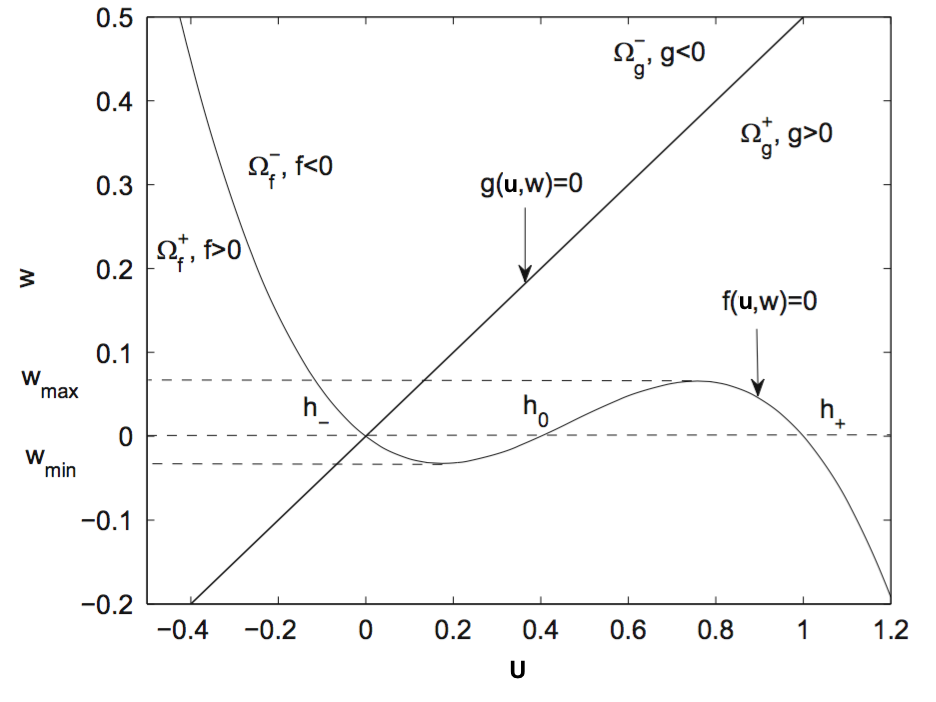
\includegraphics[width=0.8\textwidth]{images/PhasediagramFN.png}
    \caption{$u$ and $w$-phase plane diagram for the FN model. Nullcline intersection points are indicated as $h_-$, $h_0$ and $h_+$. \citep{ecg}}
    \label{fig2b.1}
\end{figure}
To fully understand the behaviour of equation \ref{eqGFN} a phase analysis is necessary. As shown in figure \ref{fig2b.1}, the nullcline $f(u,w)=0$ is a cubic like function with 3 distinct zeros: $h_-$, $h_0$ and $h_+$. The nullcline $g(u,w)=0$ has only one intersection point which is an equilibrium point of the system. As the phase plane trajectory passes across the nullclines it will attempt to move towards this equilibrium point. By choosing various initial conditions, equation parameters and applied current ($\hat I_a$), the generalised FN equation (equation \ref{eqGFN}) shows greatly varying dynamics. \par
For the generalised FN system, stability exists when the phase plane trajectory lies on the upper ($h_+$) or lower ($h_-$) branch of the $f=0$ nullcine while there is instability when the trajectory lies on the middle ($h_0$) branch. There are 3 main situations when manipulating the applied current; when $\hat I_a = 0$, $\hat I_a > 0$, and when $\hat I_a$ is pulsed.

    \subsubsection{Generalised FN with Zero Applied Current}
    With zero applied current the parameters of the equation have a major impact in the phase plane trajectory (figure \ref{fig2b.2}).\par
    If the initial condition $u_0 < h_0$ holds then a sub-threshold response is witnessed as $v$ returns directly to the equilibrium point via the lower branch. This is because within the region $\Omega _{f}^{-} \Omega _{g}^{-}$ the trajectory is above the nullcline $g=0$ which forces the return down $h_-$ to the equilibrium point. Similarly if the parameters start in the $\Omega _{f}^{-} \Omega _{g}^{+}$ region then $g>0$ so initially increases the trajectory across $g=0$ back into the $\Omega _{f}^{-} \Omega _{g}^{-}$ region. \par
    If, however, the initial condition $u_0>h_0$ is chosen then a single action potential can be observed. A clear excitation phase is seen when the trajectory tends to the upper branch. This is followed by a very brief plateau as the trajectory lingers on the upper branch. The gating variable $w$ evolves into an approximate constant, driving the trajectory across the $g=0$ nullcline towards the lower branch, this mimics the recovery phase. The trajectory then relaxes down the lower branch to the equilibrium point. \par
    Alternative to these stable equilibrium situations an unstable equilibrium can be formed. This forms a limit cycle due to periodic solutions. This occurs when the equilibrium point lies on the middle branch as the trajectory of initial excitation starts a second excitation phase generating periodic action potentials. This scenario could potentially be of use in simulating the limited periodic cycles observed on SAN cells.
    \begin{SCfigure}[0.7][h!]
        \centering
        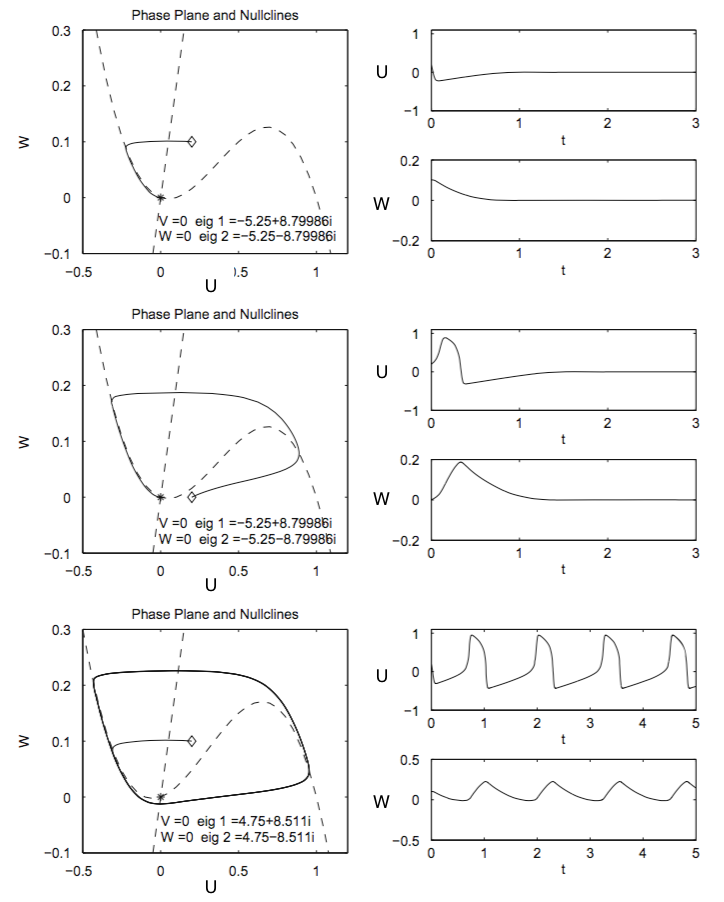
\includegraphics[width=0.65\textwidth]{images/I0cycles.png}
        \caption{Generalised FN model with $\hat I_a = 0, \epsilon=0.01$. For top and middle $f(u,w) = u(u-0.1)(1-u)-w, g(u,w)=u-w/2$. For bottom $f(u,w) = u(u+0.1)(1-u)-w, g(u,w)=u-w/2$. Equilibrium point is marked with a black star, start position is marked with a white diamond. The associated solutions are to the right of the phase diagrams. \citep{ecg}}
        \label{fig2b.2}
    \end{SCfigure}
    \subsubsection{Generalised FN with a Non-zero Applied Current}
    With a small applied constant current an unstable equilibrium can be formed with a periodic limit cycle, similar to the one shown in the bottom panel of figure \ref{fig2b.2}. This is achieved by shifting the $f=0$ nullcline upwards, moving the equilibrium point closer to the upper branch (however still on the middle branch) forcing it to behave as a source point. This yields a periodic action potential where the plateau period can be manipulated by adjusting the equation parameters. \par
    If the applied current is too high the equilibrium point tips over the peak of the $f=0$ nullcline onto the upper branch causing it to behave as a sink point, this attracts the trajectory.
    \begin{SCfigure}[0.7][h!]
        \centering
        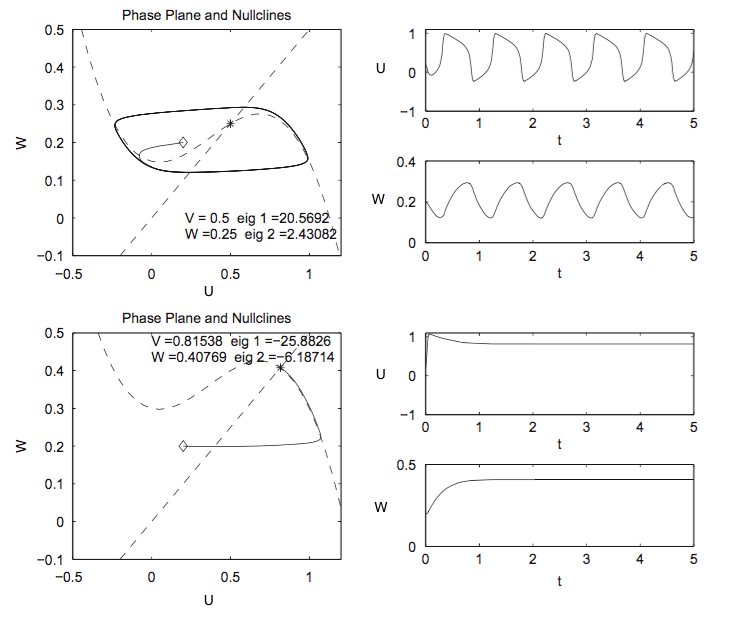
\includegraphics[width=0.63\textwidth]{images/Iposcycles.png}
        \caption{The effects of positive applied potential on the phase plane trajectories of the general FN equation $f(u,w)=u(u-0.1)(1-u)-w, g(u,w)=u-2w$, with $\epsilon=0.01$. Top $\hat I_a = 0.15$, bottom $\hat I_a =0.3$. \citep{ecg}}
        \label{fig2b.3}
    \end{SCfigure}
    \subsubsection{Generalised FN with a Pulsed Non-zero Applied Current}
    In the previous examples a constant applied current has been used. A more physiologically accurate method is to use a pulsed applied current. This simulates the activation of the action potential via a neighbouring cell's pulse or an external stimulus such as a nerve. In this situation the duration that the current pulse is applied for has a significant impact. The applied current pulse temporarily shifts the $f=0$ nullcline upwards (if $\hat I_a >0$) or downwards ($\hat I_a <0$) causing the equilibrium point to shift, this forces the trajectory towards to closest branch. When the pulse is turned off the nullcline returns to the original position. At this time the trajectory is at a point (if correct times and parameters are chosen) which belongs to the excitable region causing an action potential. \par 
    For the generalised FN equation, $f(u,w)=u(u-0.1)(1-u)-w,  g(u,w)=u-w/2$, a positive and negative pulse causes a cathode make and anode break mechanism respectively. A 'make' occurs when an applied current is turned on and a 'break' is where an applied current is turned off. Cathode and anode refer to a negative and positive applied current respectively. The anode break is shown in figure \ref{fig2b.3}. Additional mechanism, known as cathode break and anode make, are observed in more complex systems within cardiac domains. 
    \begin{SCfigure}[0.7][h!]
        \centering
        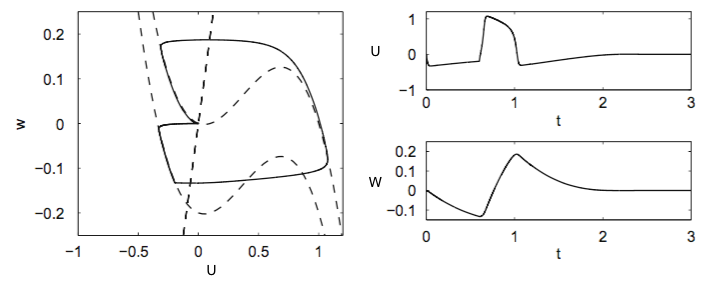
\includegraphics[width=0.65\textwidth]{images/Iperiod.png}
        \caption{A current pulse of $\hat I_a=-0.2$ for 0.6 ms causing an anode break. This action potential is an accurate simulation of an atrial conduction cell. \citep{ecg}}
        \label{fig2b.4}
    \end{SCfigure}
\subsection{Advanced Models}
More advanced models exist that take into account more complex parameters of the system such as rotational anisotropy, conduction fibre structure, cell shape, and the inhomogeneous nature of the intra and extra cellular mediums. \par
The bidomain model is derived from a one dimensional model of an electrical cable. The biodomain model takes the average of all the properties of the cells in the medium rather than modelling each cell individually \citep{bidomain}. The main problem the bidomain model tackles is the anisotropy of electrical conductivity. Within cardiac tissue there is unequal anisotropy ratios for the conductivities parallel and perpendicular to the fibres within the intra and extra cellular mediums. For cardiac tissues the ratio for intracellular space is 10:1, while in extracellular space it is 5:2 \citep{bidomainans}. This anisotropy can effect the action potential in many ways such as the distribution of the transmembrane potential \citep{disttrans}, the magnetic field produced by the propagating wave \citep{magfield}, and the effect of electric shocks on the transmembrane potential \citep{shocks}. \par 
Although detailed, this model is also mathematically cumbersome with the average simulation taking up to 2 days on a 32 processor computer \citep{monodomain}. It is regularly simplified by removing the unequal anisotropy of the intra and extra-cellular domains, this is known as the monodomain model \citep{monodomain}. The monodomain model is more computationally lightweight and does ignore the large difference in anisotropy of the mediums, however, the propagation of activation has been reported to being only 2\% faster for the monodomain model \citep{monodomain}. It has also been reported by the same group that ECGs computed using both models are visually indistinguishable suggesting that this anisotropy can be ignored and effective simulation can still be achieved. The same argument has been used for ignoring the anisotropy in cubic-like models.
\begin{figure}[H]
    \centering
    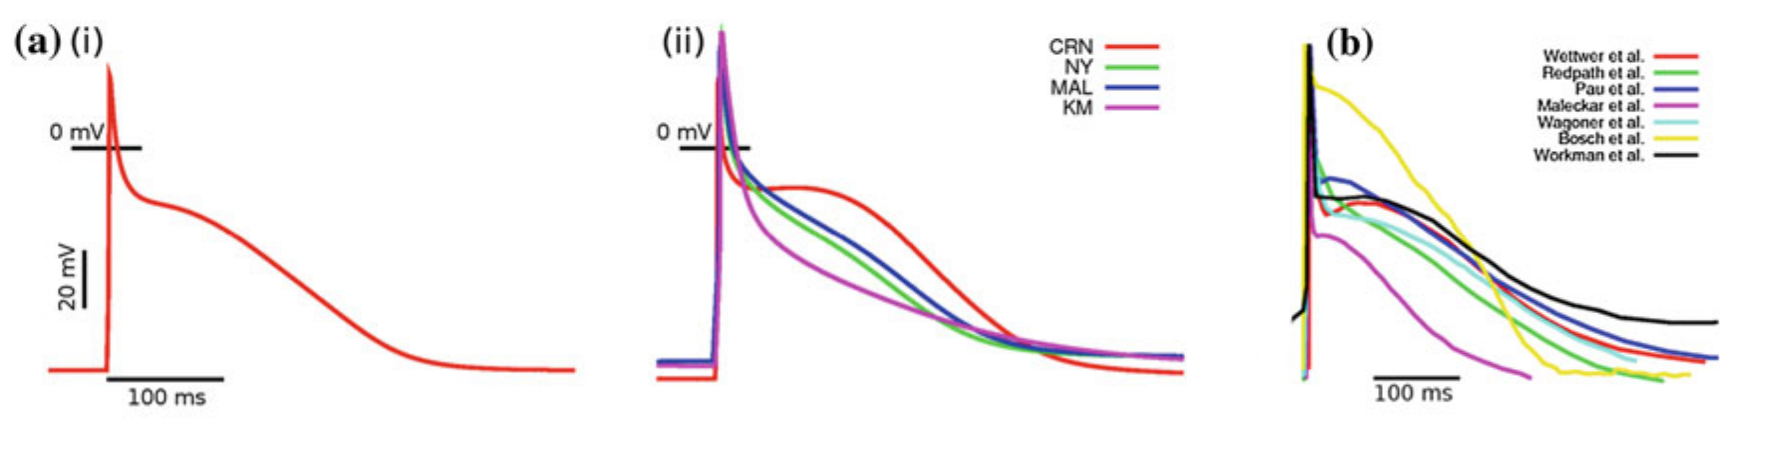
\includegraphics[width=0.9\textwidth]{images/APmodels.png}
    \caption{The (a) panels show a variety of advanced models and the (b) panels show a collection of experimental measurements. (i) shows one of the most detailed models known as the MCZ model by M. Colman \citep{phdpaper}. It is clear that experimental and modelled potentials vary significantly. \citep{phdpaper}}
    \label{fig2b.5}
\end{figure}